\chapter{Theoretical Background}
\label{chapter:theoretical_background}

This chapter introduces the theoretical background which motivates this search performed in the thesis. 
The discussion begins with the Standard Model~(SM), which provides the current theoretical framework for describing elementary particles and their interactions. 
The limitations of the SM are then summarised, followed by a discussion of several possible extensions beyond the SM. 
Particular emphasis is placed on leptoquark models, which provide a direct connection between the quark and lepton sectors and motivate the experimental search presented in this thesis.

\section{The Standard Model}
\label{sec:sm}

The Standard Model~(SM) is a relativistic quantum field theory describing the known elementary particles and their strong, weak, and electromagnetic interactions. 
Its structure is determined by local gauge invariance under
\begin{align}
    SU(3)_{C} \times SU(2)_{L} \times U(1)_{Y}.
\end{align}
The group $SU(3)_{C}$ describes the colour symmetry of the strong interaction, while $SU(2)_{L} \times U(1)_{Y}$ describes the electroweak interaction~\cite{Glashow1961,Weinberg1967,Salam1968}. 
In quantum field theory, particles are classified not only by their mass and spin, but also by their transformation properties under these gauge symmetries. 
Particles with half-integer spin are fermions and obey Fermi--Dirac statistics, while particles with integer spin are bosons and obey Bose--Einstein statistics~\cite{Pauli1940}. 
The matter particles of the SM are spin-$1/2$ fermions, the interaction carriers are spin-$1$ gauge bosons, and the Higgs boson is a spin-$0$ scalar boson.

The minimal SM Lagrangian used here is constructed from the SM field content and is invariant under the local gauge group. Therefore, instead of introducing the Lagrangian as an isolated expression, this section first summarises the field content and gauge quantum numbers of the SM. The principle of local gauge invariance is then introduced, followed by the gauge transformations of the strong sector, based on $SU(3)_{C}$, and of the electroweak sector, based on $SU(2)_{L}\times U(1)_{Y}$. The covariant derivative and field-strength tensors are then constructed from these symmetries, leading to the full SM Lagrangian.
Finally, electroweak symmetry breaking and the generation of fermion masses are discussed.


\subsection{Particle content and gauge group of the SM}
\label{subsec:sm_particle_content}

The gauge quantum numbers of a field specify how it transforms under the SM gauge group. 
In this thesis, the electric charge is written as
\begin{align}
    Q = T^{3} + Y,
    \label{eq:electric_charge_relation}
\end{align}
where $T^{3}$ is the third component of weak isospin and $Y$ is the weak hypercharge. 
This convention is used throughout the thesis.

For each generation, the SM fermions are arranged as
\begin{align}
    Q_{L}^{i}
    =
    \begin{pmatrix}
        u_{L}^{i} \\
        d_{L}^{i}
    \end{pmatrix}
    &\sim
    (3,2,1/6),
    &
    u_{R}^{i}
    &\sim
    (3,1,2/3),
    &
    d_{R}^{i}
    &\sim
    (3,1,-1/3),
    \\
    L_{L}^{i}
    =
    \begin{pmatrix}
        \nu_{L}^{i} \\
        e_{L}^{i}
    \end{pmatrix}
    &\sim
    (1,2,-1/2),
    &
    e_{R}^{i}
    &\sim
    (1,1,-1),
    \label{eq:sm_fermion_representations}
\end{align}
where $i=1,2,3$ is the generation index, and the notation denotes the representation under
$SU(3)_{C}\times SU(2)_{L}\times U(1)_{Y}$, which are the QCD representation, the weak isospin representation and the weak hypercharge, respectively.
In the minimal SM, no right-handed neutrino field is included. 
The scalar sector contains one complex Higgs doublet,
\begin{align}
    \Phi
    =
    \begin{pmatrix}
        \phi^{+} \\
        \phi^{0}
    \end{pmatrix}
    \sim
    (1,2,1/2).
    \label{eq:higgs_doublet_representation}
\end{align}

The gauge bosons are associated with the generators of the three gauge groups. 
The eight gluon fields $G_{\mu}^{a}$, with $a=1,\ldots,8$, are associated with $SU(3)_{C}$. 
The three weak gauge fields $W_{\mu}^{I}$, with $I=1,2,3$, are associated with $SU(2)_{L}$. 
The hypercharge gauge field $B_{\mu}$ is associated with $U(1)_{Y}$. 
Before electroweak symmetry breaking, $W_{\mu}^{1}$, $W_{\mu}^{2}$, $W_{\mu}^{3}$, and $B_{\mu}$ are gauge eigenstates. 
After electroweak symmetry breaking, they are reorganised into the physical electroweak bosons $W^{\pm}$, $Z$, and $\gamma$.

The main particle content of the SM is summarised in Table~\ref{tab:sm_particles}. 
For fermions and the Higgs boson, the table lists the corresponding electroweak quantum numbers using the convention in Eq.~\eqref{eq:electric_charge_relation}. 
For gauge bosons, the entries describe their gauge fields and the electric charges of the physical states where appropriate.

\begin{table}[htbp]
    \centering
    \caption[Standard Model particle content]{
    Particle content of the SM and the corresponding spin and electroweak
    quantum numbers.
    For fermions and the Higgs doublet, $T^{3}$ and $Y$ denote the third
    component of weak isospin and the weak hypercharge, respectively, with
    the electric charge defined as $Q=T^{3}+Y$.
    For gauge bosons, only the electric charges of the physical states after
    electroweak symmetry breaking are shown.
    }
    \label{tab:sm_particles}
    \scriptsize
    \resizebox{\textwidth}{!}{
    \begin{tabular}{ccccccccc}
        \toprule
        \multirow{2}{*}{Category}
        & \multirow{2}{*}{Type}
        & \multicolumn{3}{c}{Generation}
        & \multirow{2}{*}{Spin}
        & \multicolumn{3}{c}{Quantum numbers} \\
        & & 1st & 2nd & 3rd & & $T^{3}$ & $Y$ & $Q$ \\
        \midrule

        \multirow{5}{*}{Fermion}
        & Left-handed quark
        & $\begin{array}{c} u_{L} \\ d_{L} \end{array}$
        & $\begin{array}{c} c_{L} \\ s_{L} \end{array}$
        & $\begin{array}{c} t_{L} \\ b_{L} \end{array}$
        & $1/2$
        & $\begin{array}{c} +1/2 \\ -1/2 \end{array}$
        & $1/6$
        & $\begin{array}{c} +2/3 \\ -1/3 \end{array}$ \\

        & Right-handed up-type quark
        & $u_{R}$
        & $c_{R}$
        & $t_{R}$
        & $1/2$
        & $0$
        & $2/3$
        & $+2/3$ \\

        & Right-handed down-type quark
        & $d_{R}$
        & $s_{R}$
        & $b_{R}$
        & $1/2$
        & $0$
        & $-1/3$
        & $-1/3$ \\

        \cmidrule(lr){2-9}

        & Left-handed lepton
        & $\begin{array}{c} \nu_{eL} \\ e_{L} \end{array}$
        & $\begin{array}{c} \nu_{\mu L} \\ \mu_{L} \end{array}$
        & $\begin{array}{c} \nu_{\tau L} \\ \tau_{L} \end{array}$
        & $1/2$
        & $\begin{array}{c} +1/2 \\ -1/2 \end{array}$
        & $-1/2$
        & $\begin{array}{c} 0 \\ -1 \end{array}$ \\

        & Right-handed charged lepton
        & $e_{R}$
        & $\mu_{R}$
        & $\tau_{R}$
        & $1/2$
        & $0$
        & $-1$
        & $-1$ \\

        \midrule

        \multirow{4}{*}{Gauge boson}
        & Gluon
        & \multicolumn{3}{c}{$g^{a}$, $a=1,\ldots,8$}
        & $1$
        & --
        & --
        & $0$ \\

        & Photon
        & \multicolumn{3}{c}{$\gamma$}
        & $1$
        & --
        & --
        & $0$ \\

        & Charged weak boson
        & \multicolumn{3}{c}{$W^{\pm}$}
        & $1$
        & --
        & --
        & $\pm1$ \\

        & Neutral weak boson
        & \multicolumn{3}{c}{$Z$}
        & $1$
        & --
        & --
        & $0$ \\

        \midrule

        Scalar field
        & Higgs doublet
        & \multicolumn{3}{c}{
            $\begin{array}{c}
                \phi^{+} \\
                \phi^{0}
            \end{array}$
        }
        & $0$
        & $\begin{array}{c} +1/2 \\ -1/2 \end{array}$
        & $1/2$
        & $\begin{array}{c} +1 \\ 0 \end{array}$ \\

        \bottomrule
    \end{tabular}
    }
\end{table}

The quantum numbers listed above determine which interactions each field can have. 
They also determine which terms can be written in the SM Lagrangian. 
For example, explicit Dirac mass terms for charged fermions are not gauge invariant before electroweak symmetry breaking, because the left- and right-handed fermions transform differently under $SU(2)_{L}\times U(1)_{Y}$. 
Fermion masses instead arise from gauge-invariant Yukawa interactions with the Higgs field.


\subsection{Local gauge invariance}
\label{subsec:local_gauge_invariance}

The guiding principle in constructing the SM is local gauge invariance. 
A global transformation acts in the same way at every point in spacetime, while a local gauge transformation depends on the spacetime coordinate $x$. 
For a field $\psi(x)$ transforming under a gauge group with generators $T^{A}$, a generic local transformation is
\begin{align}
    \psi(x)
    \rightarrow
    \psi'(x)
    =
    U(x)\psi(x),
    \qquad
    U(x)
    =
    \exp\left[i\alpha^{A}(x)T^{A}\right].
    \label{eq:generic_local_transformation}
\end{align}
Here $\alpha^{A}(x)$ are arbitrary real, spacetime-dependent gauge parameters. 
They specify how the field is transformed locally along each generator $T^{A}$ of the gauge group, and the repeated index $A$ is summed over all generators.

The ordinary derivative of the transformed field is
\begin{align}
    \partial_{\mu}\psi'(x)
    =
    U(x)\partial_{\mu}\psi(x)
    +
    \left(\partial_{\mu}U(x)\right)\psi(x).
    \label{eq:ordinary_derivative_transformation}
\end{align}
The second term in Eq.~\eqref{eq:ordinary_derivative_transformation} shows that $\partial_{\mu}\psi$ does not transform in the same way as $\psi$. 
Therefore, the kinetic term constructed using the ordinary derivative is not invariant under a local gauge transformation.

To restore local gauge invariance, the ordinary derivative is promoted to a covariant derivative $D_{\mu}$ satisfying
\begin{align}
    D_{\mu}\psi(x)
    \rightarrow
    D'_{\mu}\psi'(x)
    =
    U(x)D_{\mu}\psi(x).
    \label{eq:covariant_derivative_requirement}
\end{align}
This requirement introduces gauge fields. 
The gauge fields are therefore not added by hand as arbitrary new particles; they are required in order to compare fields at neighbouring spacetime points in a way that is independent of the local gauge convention. 
The following subsections describe how this principle is realised for the strong and electroweak gauge sectors of the SM.


\subsection{The $SU(3)_{C}$ gauge sector}
\label{subsec:su3c_gauge_sector}

The strong interaction is described by quantum chromodynamics~(QCD), a gauge theory based on the colour group $SU(3)_{C}$. 
Quark fields transform as colour triplets, while leptons and the Higgs field are colour singlets. 
For a colour triplet quark field $q(x)$, the local $SU(3)_{C}$ transformation is
\begin{align}
    q(x)
    \rightarrow
    q'(x)
    =
    U_{C}(x)q(x),
    \qquad
    U_{C}(x)
    =
    \exp\left[
        i\alpha_{C}^{a}(x)\frac{\lambda^{a}}{2}
    \right],
    \label{eq:su3c_matter_transformation}
\end{align}
where $\lambda^{a}$ are the Gell-Mann matrices and $a=1,\ldots,8$. 
The corresponding gauge fields are the eight gluon fields $G_{\mu}^{a}$.

It is useful to introduce the matrix-valued gluon field
\begin{align}
    G_{\mu}(x)
    =
    G_{\mu}^{a}(x)\frac{\lambda^{a}}{2}.
    \label{eq:gluon_field_matrix}
\end{align}
With the convention
\begin{align}
    D_{\mu}
    =
    \partial_{\mu}
    -
    ig_{s}G_{\mu}^{a}\frac{\lambda^{a}}{2},
    \label{eq:su3c_covariant_derivative}
\end{align}
where $g_{s}$ is the strong coupling constant, the gluon field transforms as
\begin{align}
    G_{\mu}(x)
    \rightarrow
    G'_{\mu}(x)
    =
    U_{C}(x)G_{\mu}(x)U_{C}^{\dagger}(x)
    -
    \frac{i}{g_{s}}
    \left(\partial_{\mu}U_{C}(x)\right)U_{C}^{\dagger}(x).
    \label{eq:su3c_gauge_field_transformation}
\end{align}
This transformation law ensures that $D_{\mu}q$ transforms in the same way as $q$ under local $SU(3)_{C}$ transformations.

The $SU(3)_{C}$ field-strength tensor is
\begin{align}
    G_{\mu\nu}^{a}
    =
    \partial_{\mu}G_{\nu}^{a}
    -
    \partial_{\nu}G_{\mu}^{a}
    +
    g_{s}f^{abc}G_{\mu}^{b}G_{\nu}^{c},
    \label{eq:su3c_field_strength}
\end{align}
where $f^{abc}$ are the structure constants of $SU(3)$, defined by the commutation relation
\begin{align}
    \left[
        \frac{\lambda^{a}}{2},
        \frac{\lambda^{b}}{2}
    \right]
    =
    i f^{abc}\frac{\lambda^{c}}{2}.
    \label{eq:su3c_structure_constants}
\end{align}
The last term in Eq.~\eqref{eq:su3c_field_strength} arises from the non-Abelian nature of $SU(3)_{C}$. 
It gives rise to gluon self-interactions, which are a defining feature of QCD and are essential for asymptotic freedom at high energies and confinement at low energies.


\subsection{The electroweak gauge sector}
\label{subsec:electroweak_gauge_sector}

Before electroweak symmetry breaking, the weak and electromagnetic interactions are described together by the gauge group $SU(2)_{L}\times U(1)_{Y}$~\cite{Glashow1961,Weinberg1967,Salam1968}. 
The $SU(2)_{L}$ factor is the non-Abelian weak-isospin gauge symmetry, while the $U(1)_{Y}$ factor is the Abelian hypercharge gauge symmetry. 
They are introduced separately below, but the physical photon and $Z$ boson arise only after electroweak symmetry breaking, when the neutral fields $W_{\mu}^{3}$ and $B_{\mu}$ mix.


\subsubsection{The $SU(2)_{L}$ gauge transformation}
\label{subsec:su2l_transformation}

The $SU(2)_{L}$ gauge symmetry acts on left-handed fermion doublets and on the Higgs doublet:
\begin{align}
    Q_{L}^{i},
    \quad
    L_{L}^{i},
    \quad
    \Phi.
\end{align}
For an $SU(2)_{L}$ doublet $\chi(x)$, the local transformation is
\begin{align}
    \chi(x)
    \rightarrow
    \chi'(x)
    =
    U_{L}(x)\chi(x),
    \qquad
    U_{L}(x)
    =
    \exp\left[
        i\alpha^{I}(x)\frac{\tau^{I}}{2}
    \right],
    \label{eq:su2l_matter_transformation}
\end{align}
where $\tau^{I}$ are the Pauli matrices and $I=1,2,3$. 
The right-handed charged fermions $u_{R}^{i}$, $d_{R}^{i}$, and $e_{R}^{i}$ are singlets under $SU(2)_{L}$ and therefore have $T_{L}^{I}=0$.

The three gauge fields associated with $SU(2)_{L}$ are denoted by $W_{\mu}^{I}$. 
They can be written in matrix form as
\begin{align}
    W_{\mu}(x)
    =
    W_{\mu}^{I}(x)\frac{\tau^{I}}{2}.
    \label{eq:weak_gauge_field_matrix}
\end{align}
With the convention
\begin{align}
    D_{\mu}
    =
    \partial_{\mu}
    -
    igW_{\mu}^{I}\frac{\tau^{I}}{2},
    \label{eq:su2l_covariant_derivative}
\end{align}
where $g$ is the $SU(2)_{L}$ coupling constant, the weak gauge field transforms as
\begin{align}
    W_{\mu}(x)
    \rightarrow
    W'_{\mu}(x)
    =
    U_{L}(x)W_{\mu}(x)U_{L}^{\dagger}(x)
    -
    \frac{i}{g}
    \left(\partial_{\mu}U_{L}(x)\right)U_{L}^{\dagger}(x).
    \label{eq:su2l_gauge_field_transformation}
\end{align}
This transformation law is the non-Abelian generalisation of the Abelian gauge-field transformation. 
The matrix structure reflects the fact that the $SU(2)_{L}$ generators do not commute.

The $SU(2)_{L}$ field-strength tensor is
\begin{align}
    W_{\mu\nu}^{I}
    =
    \partial_{\mu}W_{\nu}^{I}
    -
    \partial_{\nu}W_{\mu}^{I}
    +
    g\epsilon^{IJK}W_{\mu}^{J}W_{\nu}^{K}.
    \label{eq:su2l_field_strength}
\end{align}
The last term arises from the non-Abelian nature of $SU(2)_{L}$ and leads to self-interactions among weak gauge bosons.


\subsubsection{The $U(1)_{Y}$ gauge transformation}
\label{subsec:u1y_transformation}

The $U(1)_{Y}$ gauge symmetry is the Abelian part of the electroweak gauge group. 
Its corresponding gauge charge is the weak hypercharge $Y$, which determines how each field transforms under a local $U(1)_{Y}$ phase rotation. 
For a field $\psi(x)$ with hypercharge $Y$, the local $U(1)_{Y}$ transformation is
\begin{align}
    \psi(x)
    \rightarrow
    \psi'(x)
    =
    \exp\left[iY\beta(x)\right]\psi(x),
    \label{eq:u1y_matter_transformation}
\end{align}
where $\beta(x)$ is a spacetime-dependent transformation parameter. 
The corresponding gauge field is the hypercharge field $B_{\mu}$. 
With the convention
\begin{align}
    D_{\mu}
    =
    \partial_{\mu}
    -
    ig'YB_{\mu},
    \label{eq:u1y_covariant_derivative}
\end{align}
the gauge field transforms as
\begin{align}
    B_{\mu}(x)
    \rightarrow
    B'_{\mu}(x)
    =
    B_{\mu}(x)
    +
    \frac{1}{g'}\partial_{\mu}\beta(x).
    \label{eq:u1y_gauge_field_transformation}
\end{align}
This transformation ensures that $D_{\mu}\psi$ transforms in the same way as $\psi$.

The hypercharge assignments in Table~\ref{tab:sm_particles} are chosen so that the electric charge is obtained from Eq.~\eqref{eq:electric_charge_relation}. 
For the left-handed lepton doublet, $Y=-1/2$. 
The upper component has $T^{3}=+1/2$ and therefore $Q=0$, corresponding to the neutrino. 
The lower component has $T^{3}=-1/2$ and therefore $Q=-1$, corresponding to the charged lepton. 
Similarly, the left-handed quark doublet has $Y=1/6$, giving charges $+2/3$ and $-1/3$ for the up- and down-type components.

Because $U(1)_{Y}$ is Abelian, the corresponding field-strength tensor is
\begin{align}
    B_{\mu\nu}
    =
    \partial_{\mu}B_{\nu}
    -
    \partial_{\nu}B_{\mu}.
    \label{eq:u1y_field_strength}
\end{align}
There is no self-interaction term involving two $B_{\mu}$ fields in $B_{\mu\nu}$.
Although $U(1)_{Y}$ is Abelian, it should not be identified with the electromagnetic gauge symmetry $U(1)_{\mathrm{em}}$. 
Before electroweak symmetry breaking, the corresponding gauge field is the hypercharge field $B_{\mu}$ rather than the photon field. 
The electromagnetic gauge symmetry appears only after electroweak symmetry breaking, when $B_{\mu}$ mixes with the neutral weak gauge field $W_{\mu}^{3}$ to form the photon and the $Z$ boson.


\subsection{Covariant derivative and gauge field strengths}
\label{subsec:covariant_derivative_field_strengths}

Combining the three gauge symmetries, the covariant derivative acting on a generic SM field can be written as
\begin{align}
    D_{\mu}
    =
    \partial_{\mu}
    -
    ig_{s}G_{\mu}^{a}T_{C}^{a}
    -
    igW_{\mu}^{I}T_{L}^{I}
    -
    ig'YB_{\mu}.
    \label{eq:sm_covariant_derivative}
\end{align}
Here $g_{s}$, $g$, and $g'$ are the gauge couplings of $SU(3)_{C}$, $SU(2)_{L}$, and $U(1)_{Y}$, respectively. 
The matrices $T_{C}^{a}$ and $T_{L}^{I}$ are the generators acting on the particular field. 
For a colour triplet, $T_{C}^{a}=\lambda^{a}/2$, while for a colour singlet $T_{C}^{a}=0$. 
For an $SU(2)_{L}$ doublet, $T_{L}^{I}=\tau^{I}/2$, while for an $SU(2)_{L}$ singlet $T_{L}^{I}=0$. 
The value of $Y$ is the hypercharge of the field, as listed in Table~\ref{tab:sm_particles}.

The gauge kinetic terms are constructed from the field-strength tensors:
\begin{align}
    G_{\mu\nu}^{a}
    &=
    \partial_{\mu}G_{\nu}^{a}
    -
    \partial_{\nu}G_{\mu}^{a}
    +
    g_{s}f^{abc}G_{\mu}^{b}G_{\nu}^{c},
    \\
    W_{\mu\nu}^{I}
    &=
    \partial_{\mu}W_{\nu}^{I}
    -
    \partial_{\nu}W_{\mu}^{I}
    +
    g\epsilon^{IJK}W_{\mu}^{J}W_{\nu}^{K},
    \\
    B_{\mu\nu}
    &=
    \partial_{\mu}B_{\nu}
    -
    \partial_{\nu}B_{\mu}.
    \label{eq:sm_field_strengths}
\end{align}
The tensors $G_{\mu\nu}^{a}$ and $W_{\mu\nu}^{I}$ contain non-linear terms because $SU(3)_{C}$ and $SU(2)_{L}$ are non-Abelian groups. 
By contrast, $B_{\mu\nu}$ has the Abelian form because $U(1)_{Y}$ has only one generator.

\subsection{The Standard Model Lagrangian}
\label{subsec:sm_lagrangian}

The SM Lagrangian is constructed from the field content described above and is invariant under the local gauge transformations of $SU(3)_{C}\times SU(2)_{L}\times U(1)_{Y}$. 
Using the covariant derivative and field-strength tensors introduced in the previous subsections, the minimal SM Lagrangian can be written as the sum of gauge-boson kinetic terms, fermion kinetic terms, the Higgs-sector terms, and Yukawa interactions. 
Ignoring gauge-fixing terms, ghost terms, and the QCD $\theta$-term, it is written schematically as
\begin{align}
    \mathcal{L}_{\mathrm{SM}}
    =
    \mathcal{L}_{\mathrm{gauge}}
    +
    \mathcal{L}_{\mathrm{fermion}}
    +
    \mathcal{L}_{\mathrm{Higgs}}
    +
    \mathcal{L}_{\mathrm{Yukawa}}.
    \label{eq:sm_lagrangian_decomposition}
\end{align}
The four terms in Eq.~\eqref{eq:sm_lagrangian_decomposition} are fixed by Lorentz invariance, local gauge invariance, and renormalisability, once the SM field content is specified~\cite{tHooft1971,tHooftVeltman1972}.

The gauge-boson kinetic terms are
\begin{align}
    \mathcal{L}_{\mathrm{gauge}}
    =
    -
    \frac{1}{4}
    G_{\mu\nu}^{a}G^{a\mu\nu}
    -
    \frac{1}{4}
    W_{\mu\nu}^{I}W^{I\mu\nu}
    -
    \frac{1}{4}
    B_{\mu\nu}B^{\mu\nu}.
    \label{eq:sm_gauge_lagrangian}
\end{align}
Here $G_{\mu\nu}^{a}$, $W_{\mu\nu}^{I}$, and $B_{\mu\nu}$ are the field-strength tensors of $SU(3)_{C}$, $SU(2)_{L}$, and $U(1)_{Y}$, respectively. 
The indices $a=1,\ldots,8$ and $I=1,2,3$ label the generators of $SU(3)_{C}$ and $SU(2)_{L}$, and repeated Lorentz and gauge indices are summed over. 
The common factor $-1/4$ gives the conventional canonical normalisation of the gauge-boson kinetic terms. 
With this normalisation, the quadratic parts of Eq.~\eqref{eq:sm_gauge_lagrangian} describe the free propagation of the gluon, weak, and hypercharge gauge fields, while the non-Abelian parts of $G_{\mu\nu}^{a}$ and $W_{\mu\nu}^{I}$ generate self-interactions among the corresponding gauge bosons.


The fermion kinetic terms are
\begin{align}
    \mathcal{L}_{\mathrm{fermion}}
    =
    \sum_{i=1}^{3}
    \bigg[
        \bar{Q}_{L}^{i} i\gamma^{\mu}D_{\mu}Q_{L}^{i}
        +
        \bar{u}_{R}^{i} i\gamma^{\mu}D_{\mu}u_{R}^{i}
        +
        \bar{d}_{R}^{i} i\gamma^{\mu}D_{\mu}d_{R}^{i}
        +
        \bar{L}_{L}^{i} i\gamma^{\mu}D_{\mu}L_{L}^{i}
        +
        \bar{e}_{R}^{i} i\gamma^{\mu}D_{\mu}e_{R}^{i}
    \bigg].
    \label{eq:sm_fermion_lagrangian}
\end{align}
The sum runs over the three fermion generations. 
The fields $Q_{L}^{i}$ and $L_{L}^{i}$ are the left-handed quark and lepton doublets, while $u_{R}^{i}$, $d_{R}^{i}$, and $e_{R}^{i}$ are right-handed singlets under $SU(2)_{L}$. 
The Dirac adjoint is defined as $\bar{\psi}=\psi^{\dagger}\gamma^{0}$, and $\gamma^{\mu}$ are the Dirac gamma matrices. 
The covariant derivative $D_{\mu}$ contains the gauge fields and couplings appropriate to the gauge quantum numbers of each fermion field. 
Therefore, Eq.~\eqref{eq:sm_fermion_lagrangian} describes both the free propagation of fermions and their gauge interactions.

The Higgs-sector terms are
\begin{align}
    \mathcal{L}_{\mathrm{Higgs}}
    =
    (D_{\mu}\Phi)^{\dagger}(D^{\mu}\Phi)
    -
    V(\Phi),
    \qquad
    V(\Phi)
    =
    -
    \mu^{2}\Phi^{\dagger}\Phi
    +
    \lambda(\Phi^{\dagger}\Phi)^{2}.
    \label{eq:sm_higgs_lagrangian}
\end{align}
The first term is the kinetic term of the Higgs doublet and also contains the gauge interactions of the Higgs field through the covariant derivative. 
The function $V(\Phi)$ is the Higgs potential. 
With the convention used here, $\mu^{2}>0$ and $\lambda>0$. 
The condition $\lambda>0$ ensures that the potential is bounded from below, while the negative quadratic term causes the minimum of the potential to occur at a non-zero value of $\Phi^{\dagger}\Phi$. 
This leads to electroweak symmetry breaking through the Brout--Englert--Higgs mechanism~\cite{Englert1964,Higgs1964,Guralnik1964}.

The Yukawa interactions are
\begin{align}
    \mathcal{L}_{\mathrm{Yukawa}}
    =
    -
    y_{d}^{ij}\bar{Q}_{L}^{i}\Phi d_{R}^{j}
    -
    y_{u}^{ij}\bar{Q}_{L}^{i}\tilde{\Phi} u_{R}^{j}
    -
    y_{e}^{ij}\bar{L}_{L}^{i}\Phi e_{R}^{j}
    +
    \mathrm{h.c.},
    \label{eq:sm_yukawa_lagrangian}
\end{align}
where $i,j=1,2,3$ are generation indices, and $y_{u}^{ij}$, $y_{d}^{ij}$, and $y_{e}^{ij}$ are complex Yukawa coupling matrices in flavour space. 
$\mathrm{h.c.}$ denotes the Hermitian conjugate. 
The conjugate Higgs doublet is defined as
\begin{align}
    \tilde{\Phi}
    =
    i\tau^{2}\Phi^{*},
    \label{eq:higgs_conjugate_doublet}
\end{align}
where $\tau^{2}$ is the second Pauli matrix. 
The field $\tilde{\Phi}$ transforms as an $SU(2)_{L}$ doublet with hypercharge opposite to that of $\Phi$, allowing a gauge-invariant Yukawa interaction for up-type quarks. 
After electroweak symmetry breaking, the Yukawa interactions generate masses for the charged fermions. 
In the minimal SM, no right-handed neutrino field is included, and therefore no renormalisable neutrino Yukawa mass term appears in Eq.~\eqref{eq:sm_yukawa_lagrangian}.

\subsection{Electroweak symmetry breaking and the Higgs mechanism}
\label{subsec:ewsb}

The Higgs potential in Eq.~\eqref{eq:sm_higgs_lagrangian} has a minimum at a non-zero value of $\Phi^{\dagger}\Phi$. 
For the convention used in Eq.~\eqref{eq:sm_higgs_lagrangian}, the minimum satisfies $\Phi^{\dagger}\Phi=v^{2}/2$, where $v=\sqrt{\mu^{2}/\lambda}$ is the Higgs vacuum expectation value and sets the electroweak scale. 
A convenient choice of vacuum expectation value is
\begin{align}
    \langle\Phi\rangle
    =
    \frac{1}{\sqrt{2}}
    \begin{pmatrix}
        0 \\
        v
    \end{pmatrix}.
    \label{eq:higgs_vev}
\end{align}
The value of $v$ is related to the Fermi constant by $v=(\sqrt{2}G_{F})^{-1/2}\simeq 246~\GeV$~\cite{PDG2025}.

This vacuum breaks the electroweak symmetry according to
\begin{align}
    SU(2)_{L}\times U(1)_{Y}
    \rightarrow
    U(1)_{\mathrm{em}}.
    \label{eq:ewsb_breaking_pattern}
\end{align}
The unbroken symmetry is electromagnetism. 
This mass-generation mechanism for gauge bosons is the Brout--Englert--Higgs mechanism~\cite{Englert1964,Higgs1964,Guralnik1964}.

In unitary gauge, the Higgs doublet can be written as
\begin{align}
    \Phi(x)
    =
    \frac{1}{\sqrt{2}}
    \begin{pmatrix}
        0 \\
        v+h(x)
    \end{pmatrix},
    \label{eq:higgs_unitary_gauge}
\end{align}
where $h(x)$ is the physical Higgs boson field. 
Expanding the Higgs potential around the vacuum gives
\begin{align}
    V(\Phi)
    =
    V(\langle\Phi\rangle)
    +
    \frac{1}{2}m_{h}^{2}h^{2}
    +
    \lambda v h^{3}
    +
    \frac{\lambda}{4}h^{4},
    \label{eq:higgs_potential_expanded}
\end{align}
where the physical Higgs-boson mass is
\begin{align}
    m_{h}^{2}
    =
    2\lambda v^{2}
    =
    2\mu^{2}.
    \label{eq:higgs_boson_mass}
\end{align}
Unlike the $W$ and $Z$ boson masses, which are fixed at tree level by the electroweak gauge couplings and the vacuum expectation value, the Higgs-boson mass depends on the quartic coupling $\lambda$. 
Therefore, the SM does not predict the numerical value of $m_{h}$ before $\lambda$ is fixed experimentally. 
The Higgs boson was observed by the ATLAS and CMS experiments in 2012~\cite{ATLAS2012Higgs,CMS2012Higgs}. 
The observed Higgs-boson mass is approximately $125~\GeV$, corresponding to $\lambda\simeq m_{h}^{2}/(2v^{2})\simeq0.13$~\cite{ATLASCMSHiggsMass2015}.

The masses of the electroweak gauge bosons arise from the Higgs kinetic term,
\begin{align}
    (D_{\mu}\Phi)^{\dagger}(D^{\mu}\Phi),
\end{align}
after substituting the Higgs vacuum expectation value. 
It is useful to define the charged weak fields as
\begin{align}
    W_{\mu}^{\pm}
    =
    \frac{1}{\sqrt{2}}
    \left(
        W_{\mu}^{1}
        \mp
        iW_{\mu}^{2}
    \right).
    \label{eq:charged_weak_bosons}
\end{align}
The terms quadratic in the electroweak gauge fields are then
\begin{align}
    (D_{\mu}\langle\Phi\rangle)^{\dagger}
    (D^{\mu}\langle\Phi\rangle)
    =
    \frac{g^{2}v^{2}}{4}W_{\mu}^{+}W^{-\mu}
    +
    \frac{v^{2}}{8}
    \left(
        gW_{\mu}^{3}
        -
        g'B_{\mu}
    \right)^{2}.
    \label{eq:ew_gauge_boson_mass_terms}
\end{align}
The first term is the mass term of the charged weak bosons. 
The second term shows that the neutral gauge fields $W_{\mu}^{3}$ and $B_{\mu}$ mix and must be diagonalised.

The weak mixing angle is defined by
\begin{align}
    \cos\theta_{W}
    =
    \frac{g}{\sqrt{g^{2}+g'^{2}}},
    \qquad
    \sin\theta_{W}
    =
    \frac{g'}{\sqrt{g^{2}+g'^{2}}}.
    \label{eq:weak_mixing_angle}
\end{align}
The corresponding neutral mass eigenstates are
\begin{align}
    A_{\mu}
    &=
    B_{\mu}\cos\theta_{W}
    +
    W_{\mu}^{3}\sin\theta_{W},
    \\
    Z_{\mu}
    &=
    -
    B_{\mu}\sin\theta_{W}
    +
    W_{\mu}^{3}\cos\theta_{W}.
    \label{eq:electroweak_mixing}
\end{align}
The field $A_{\mu}$ is identified with the photon, while $Z_{\mu}$ is the neutral weak boson. 
The photon remains massless because it is associated with the unbroken gauge symmetry $U(1)_{\mathrm{em}}$.

The resulting gauge-boson masses are
\begin{align}
    m_{W}
    =
    \frac{1}{2}gv,
    \qquad
    m_{Z}
    =
    \frac{1}{2}\sqrt{g^{2}+g'^{2}}\,v
    =
    \frac{m_{W}}{\cos\theta_{W}},
    \qquad
    m_{\gamma}=0.
    \label{eq:ew_gauge_boson_masses}
\end{align}
Thus, the SM predicts the relation $m_{W}=m_{Z}\cos\theta_{W}$. 
Inserting $v \simeq 246~\GeV$ and the electroweak couplings gives $m_{W}\simeq80~\GeV$ and $m_{Z}\simeq91~\GeV$.
Therefore, the Higgs mechanism gives masses to the $W$ and $Z$ bosons while leaving the photon massless.

After electroweak symmetry breaking, the unbroken gauge symmetry is $U(1)_{\mathrm{em}}$, whose gauge field is the photon field $A_{\mu}$. 
At energies much below the electroweak scale, the electromagnetic interactions of charged fermions are described by quantum electrodynamics~(QED). 
For a charged fermion field $\psi$ with electric charge $Q$, the QED Lagrangian can be written as
\begin{align}
    \mathcal{L}_{\mathrm{QED}}
    =
    -
    \frac{1}{4}
    F_{\mu\nu}F^{\mu\nu}
    +
    \bar{\psi}
    \left(
        i\gamma^{\mu}D_{\mu}
        -
        m
    \right)
    \psi,
    \label{eq:qed_lagrangian}
\end{align}
where
\begin{align}
    D_{\mu}
    =
    \partial_{\mu}
    -
    ieQA_{\mu},
    \qquad
    F_{\mu\nu}
    =
    \partial_{\mu}A_{\nu}
    -
    \partial_{\nu}A_{\mu}.
    \label{eq:qed_covariant_derivative}
\end{align}
Here $e$ is the electromagnetic coupling constant, $Q$ is the electric charge of the fermion in units of $e$, and $F_{\mu\nu}$ is the electromagnetic field-strength tensor. 
Thus, QED appears as the low-energy gauge theory associated with the unbroken $U(1)_{\mathrm{em}}$ symmetry of the SM.


\subsection{Fermion masses and flavour mixing}
\label{subsec:yukawa_flavour}

The Yukawa interactions generate fermion masses after electroweak symmetry breaking. 
When the Higgs field acquires its vacuum expectation value $v$, the Yukawa coupling matrices are converted into fermion mass matrices:
\begin{align}
    M_{u}^{ij}
    =
    \frac{v}{\sqrt{2}}y_{u}^{ij},
    \qquad
    M_{d}^{ij}
    =
    \frac{v}{\sqrt{2}}y_{d}^{ij},
    \qquad
    M_{e}^{ij}
    =
    \frac{v}{\sqrt{2}}y_{e}^{ij}.
    \label{eq:fermion_mass_matrices}
\end{align}
Here $M_{u}$, $M_{d}$, and $M_{e}$ are the mass matrices of the up-type quarks, down-type quarks, and charged leptons, respectively. 
The matrices $y_{u}$, $y_{d}$, and $y_{e}$ are the corresponding dimensionless Yukawa coupling matrices, and the indices $i,j=1,2,3$ label the fermion generations. 
% Since the Yukawa matrices are in general not diagonal, the mass matrices are also not diagonal in the weak-interaction basis.

The physical fermion masses are obtained by diagonalising the mass matrices. 
In the quark sector, the up-type and down-type mass matrices are diagonalised by different rotations in flavour space. 
As a result, flavour mixing appears in the charged-current weak interaction. 
This mixing is described by the Cabibbo--Kobayashi--Maskawa~(CKM) matrix~\cite{Cabibbo1963,KobayashiMaskawa1973}. 
In the mass eigenstate basis, the charged-current interaction of quarks is
\begin{align}
    \mathcal{L}_{\mathrm{CC}}
    =
    \frac{g}{\sqrt{2}}
    \bar{u}_{L}^{i}
    \gamma^{\mu}
    V_{ij}^{\mathrm{CKM}}
    d_{L}^{j}
    W_{\mu}^{+}
    +
    \mathrm{h.c.}
    \label{eq:charged_current_ckm}
\end{align}
Here $g$ is the $SU(2)_{L}$ gauge coupling, $u_{L}^{i}$ and $d_{L}^{j}$ are the left-handed up-type and down-type quark mass eigenstates, and $W_{\mu}^{+}$ is the charged weak gauge boson. 
The matrix element $V_{ij}^{\mathrm{CKM}}$ describes the strength of the charged-current transition from the down-type quark $d^{j}$ to the up-type quark $u^{i}$. 
The matrices $\gamma^{\mu}$ are the Dirac gamma matrices, and the Hermitian-conjugate term describes the corresponding interaction involving $W_{\mu}^{-}$. 
The CKM matrix is essential for describing flavour-changing charged-current processes such as $b\rightarrow c\tau\nu$, which are relevant for the leptoquark scenarios discussed later. 
Its complex phase also provides a source of CP violation in the quark sector of the SM.

In the minimal SM, neutrino masses are absent because no right-handed neutrino fields are included and no renormalisable neutrino Yukawa interaction can be written with the minimal field content. 
This provides one of the motivations for considering extensions of the SM.


\section{Beyond the Standard Model}
\label{sec:bsm}

Although the SM has been tested with high precision and has successfully described a wide range of experimental observations, it is not a complete theory of nature. 
Several experimental and theoretical facts point to physics beyond the SM.

\subsection{Gravity and the Planck scale}
\label{subsec:gravity_planck_scale}

The SM describes the electromagnetic, weak, and strong interactions as quantum gauge field theories, but it does not include gravity. 
Gravity is instead described at macroscopic scales by general relativity. 
A complete theory of nature is therefore expected to provide a consistent quantum description of gravity and to explain its connection to the SM interactions.

The difficulty of connecting gravity with the SM appears in two related ways. 
First, quantum gravitational effects are expected to become important at the Planck scale, $M_{\mathrm{Pl}}\sim10^{19}~\GeV$. This is much higher than the electroweak scale, $v\simeq246~\GeV$.
This large separation of scales is closely related to the hierarchy problem discussed below.

Second, constructing a quantum theory of gravity is theoretically challenging. 
If general relativity is quantised perturbatively in the same way as ordinary quantum field theories, it is not renormalisable as a fundamental theory. 
This makes it difficult to combine gravity with the quantum-field-theoretic framework of the SM in a straightforward way. 
Several possible approaches to quantum gravity have been proposed, including string theory, loop quantum gravity, and asymptotic safety, although no complete theory has been experimentally confirmed.

\subsection{The hierarchy problem}
\label{subsec:hierarchy_problem}

The electroweak scale is set by the Higgs vacuum expectation value, $v\simeq246~\GeV$, and is closely related to the masses of the weak gauge bosons and the Higgs boson. 
In the SM, the Higgs-boson mass is determined at tree level by
\begin{align}
    m_{h}^{2}
    =
    2\lambda v^{2},
    \label{eq:higgs_mass_lambda}
\end{align}
where $\lambda$ is the Higgs quartic coupling. 
The observed value $m_{h}\simeq125~\GeV$ therefore corresponds to $\lambda\simeq0.13$.

The hierarchy problem arises because the Higgs mass parameter is highly sensitive to physics at very high energy scales. 
If the SM is treated as an effective theory valid up to an ultraviolet cutoff scale $\Lambda$, loop corrections to the Higgs mass can be written schematically as
\begin{align}
    m_{h,\mathrm{phys}}^{2}
    =
    m_{h,0}^{2}
    +
    \delta m_{h}^{2},
    \label{eq:higgs_mass_correction}
\end{align}
where $m_{h,0}^{2}$ is the bare Higgs mass parameter and $\delta m_{h}^{2}$ denotes the quantum correction. 
At one-loop order, the correction contains terms quadratically sensitive to the cutoff scale,
\begin{align}
    \delta m_{h}^{2}
    \sim
    \frac{\Lambda^{2}}{16\pi^{2}},
    \label{eq:higgs_quadratic_correction}
\end{align}
If the cutoff scale is close to the Planck scale, $\Lambda\sim M_{\mathrm{Pl}}\sim10^{19}~\GeV$, the magnitude of $\delta m_{h}^{2}$ is many orders of magnitude larger than the observed value $m_{h}^{2}\sim(125~\GeV)^{2}$. 
Therefore, the bare parameter $m_{h,0}^{2}$ and the quantum correction $\delta m_{h}^{2}$ must cancel each other with extremely high precision in order to leave the observed electroweak-scale Higgs mass. 
This required cancellation is known as fine-tuning.

The hierarchy problem is the question of why the electroweak scale remains so much smaller than a possible ultraviolet scale such as the Planck scale. 
It motivates many extensions of the SM, such as supersymmetry, composite Higgs models, and other scenarios in which new physics appears near the TeV scale and stabilises the Higgs mass against large ultraviolet corrections. 
More generally, the hierarchy problem provides one of the motivations for experimental searches for new particles at the TeV scale. 


\subsection{Neutrino masses}
\label{subsec:neutrino_masses}

In the minimal SM, neutrinos are massless because no right-handed neutrino fields are included and no renormalisable neutrino mass term can be written using only the SM field content. 
However, neutrino oscillation experiments have shown that neutrinos change flavour as they propagate, which requires non-zero neutrino mass differences. 
Evidence for atmospheric neutrino oscillations was reported by the Super-Kamiokande experiment~\cite{SuperK1998}, and solar neutrino flavour transformation was established by the Sudbury Neutrino Observatory~\cite{SNO2002}. 
Therefore, neutrino masses provide direct experimental evidence for physics beyond the minimal SM.

\subsection{Dark matter}
\label{subsec:dark_matter}

Astrophysical and cosmological observations indicate the existence of non-luminous matter that cannot be explained by the known particles of the SM. 
Measurements of the cosmic microwave background, for example by the Planck satellite, are well described by a cosmological model containing a significant non-baryonic dark matter component~\cite{Planck2018}. 
The SM does not contain a suitable cold dark matter candidate. 
Although neutrinos are electrically neutral and weakly interacting, their small masses and relativistic behaviour in the early universe do not provide the required cold dark matter component.

\subsection{Matter--antimatter asymmetry}
\label{subsec:baryon_asymmetry}

The observable universe contains much more matter than antimatter. 
Sakharov identified three necessary conditions for dynamically generating such a baryon asymmetry: baryon-number violation, C and CP violation, and departure from thermal equilibrium~\cite{Sakharov1967}. 
The SM contains CP violation through the CKM matrix and baryon-plus-lepton number violation through non-perturbative electroweak effects. 
However, the amount of CP violation in the SM and the nature of the electroweak phase transition are not sufficient to explain the observed baryon asymmetry of the universe~\cite{Gavela1994,Cohen1993}. 
This motivates new sources of CP violation and new dynamics in the early universe.

\subsection{The strong CP problem}
\label{subsec:strong_cp}

The most general QCD Lagrangian allows a CP-violating term of the form
\begin{align}
    \mathcal{L}_{\theta}
    =
    \theta
    \frac{g_{s}^{2}}{32\pi^{2}}
    G_{\mu\nu}^{a}
    \tilde{G}^{a\mu\nu},
    \qquad
    \tilde{G}^{a\mu\nu}
    =
    \frac{1}{2}
    \epsilon^{\mu\nu\rho\sigma}
    G_{\rho\sigma}^{a}.
    \label{eq:qcd_theta_term}
\end{align}
Here $g_{s}$ is the strong coupling constant, and $G_{\mu\nu}^{a}$ is the gluon field-strength tensor of the $SU(3)_{C}$ gauge group, with the colour index $a=1,\ldots,8$ labelling the eight gluon fields. 
The tensor $\tilde{G}^{a\mu\nu}$ is the dual field-strength tensor, defined using the totally antisymmetric Levi-Civita tensor $\epsilon^{\mu\nu\rho\sigma}$. 
The parameter $\theta$ is a dimensionless QCD vacuum angle that controls the size of this CP-violating interaction. 
The factor $g_{s}^{2}/(32\pi^{2})$ is a conventional normalisation.

The operator $G_{\mu\nu}^{a}\tilde{G}^{a\mu\nu}$ is gauge invariant and has mass dimension four, so it is allowed by the gauge symmetry and renormalisability of QCD. 
However, it violates CP symmetry. Therefore, a non-zero value of the effective QCD vacuum angle would lead to CP violation in the strong interaction.

This term would contribute to the electric dipole moment of the neutron. 
Experimental limits on the neutron electric dipole moment strongly constrain the effective QCD vacuum angle $\bar{\theta}$~\cite{Baker2006}. 
The effective parameter $\bar{\theta}$ includes both the QCD vacuum angle $\theta$ and phases from the quark mass matrix. 
The absence of observable strong CP violation, despite the fact that such a term is allowed by the SM gauge symmetries, is known as the strong CP problem.


\subsection{Flavour anomalies and lepton flavour universality}
\label{subsec:flavour_anomalies}

The flavour structure of the SM is mainly determined by the Yukawa matrices. 
After electroweak symmetry breaking, these matrices generate the fermion mass matrices; their eigenvalues determine the fermion masses, while the mismatch between the diagonalisation of the up- and down-type quark mass matrices gives rise to quark flavour mixing through the CKM matrix.

Although the SM accommodates the observed masses and mixing angles, it does not explain their hierarchical pattern or their origin. 
Precision measurements in flavour physics therefore provide sensitive probes of possible physics beyond the SM.

A key property of the SM is lepton flavour universality~(LFU), which means that the electroweak gauge interactions couple equally to the three charged-lepton generations, apart from effects due to their different masses. 
Semileptonic $B$-meson decays provide precise tests of LFU by comparing decay rates involving different charged leptons. 
In charged-current transitions of the form $b\rightarrow c\ell\nu$, the commonly studied ratios are
\begin{align}
    R(D^{(*)})
    =
    \frac{
        \mathcal{B}(\bar{B}\rightarrow D^{(*)}\tau\bar{\nu}_{\tau})
    }{
        \mathcal{B}(\bar{B}\rightarrow D^{(*)}\ell\bar{\nu}_{\ell})
    },
    \qquad
    \ell=e,\mu.
    \label{eq:rd_rdstar_definition}
\end{align}
These observables compare decays involving a $\tau$ lepton with the corresponding decays involving light charged leptons.

Neutral-current transitions of the form $b\rightarrow s\ell^{+}\ell^{-}$ can be tested through ratios such as
\begin{align}
    R(K^{(*)})
    =
    \frac{
        \mathcal{B}(B\rightarrow K^{(*)}\mu^{+}\mu^{-})
    }{
        \mathcal{B}(B\rightarrow K^{(*)}e^{+}e^{-})
    }.
    \label{eq:rk_rkstar_definition}
\end{align}
These ratios compare final states with muon pairs and electron pairs. 
Recent measurements of $R(K)$ and $R(K^{*})$ are compatible with SM predictions~\cite{LHCbRK2022,LHCbRKstar2022}. 
However, measurements of $R(D)$ and $R(D^{*})$ continue to show tensions with SM predictions. 
The HFLAV CKM 2025 average gives a combined discrepancy of about $3.8\sigma$ with respect to the SM prediction~\cite{HFLAV2025RDstar} as shown in Figure~\ref{fig:HFLAV2025}. 
These observables remain important motivations for models that couple differently to different lepton generations.

\begin{figure} [htbp]
    \centering
    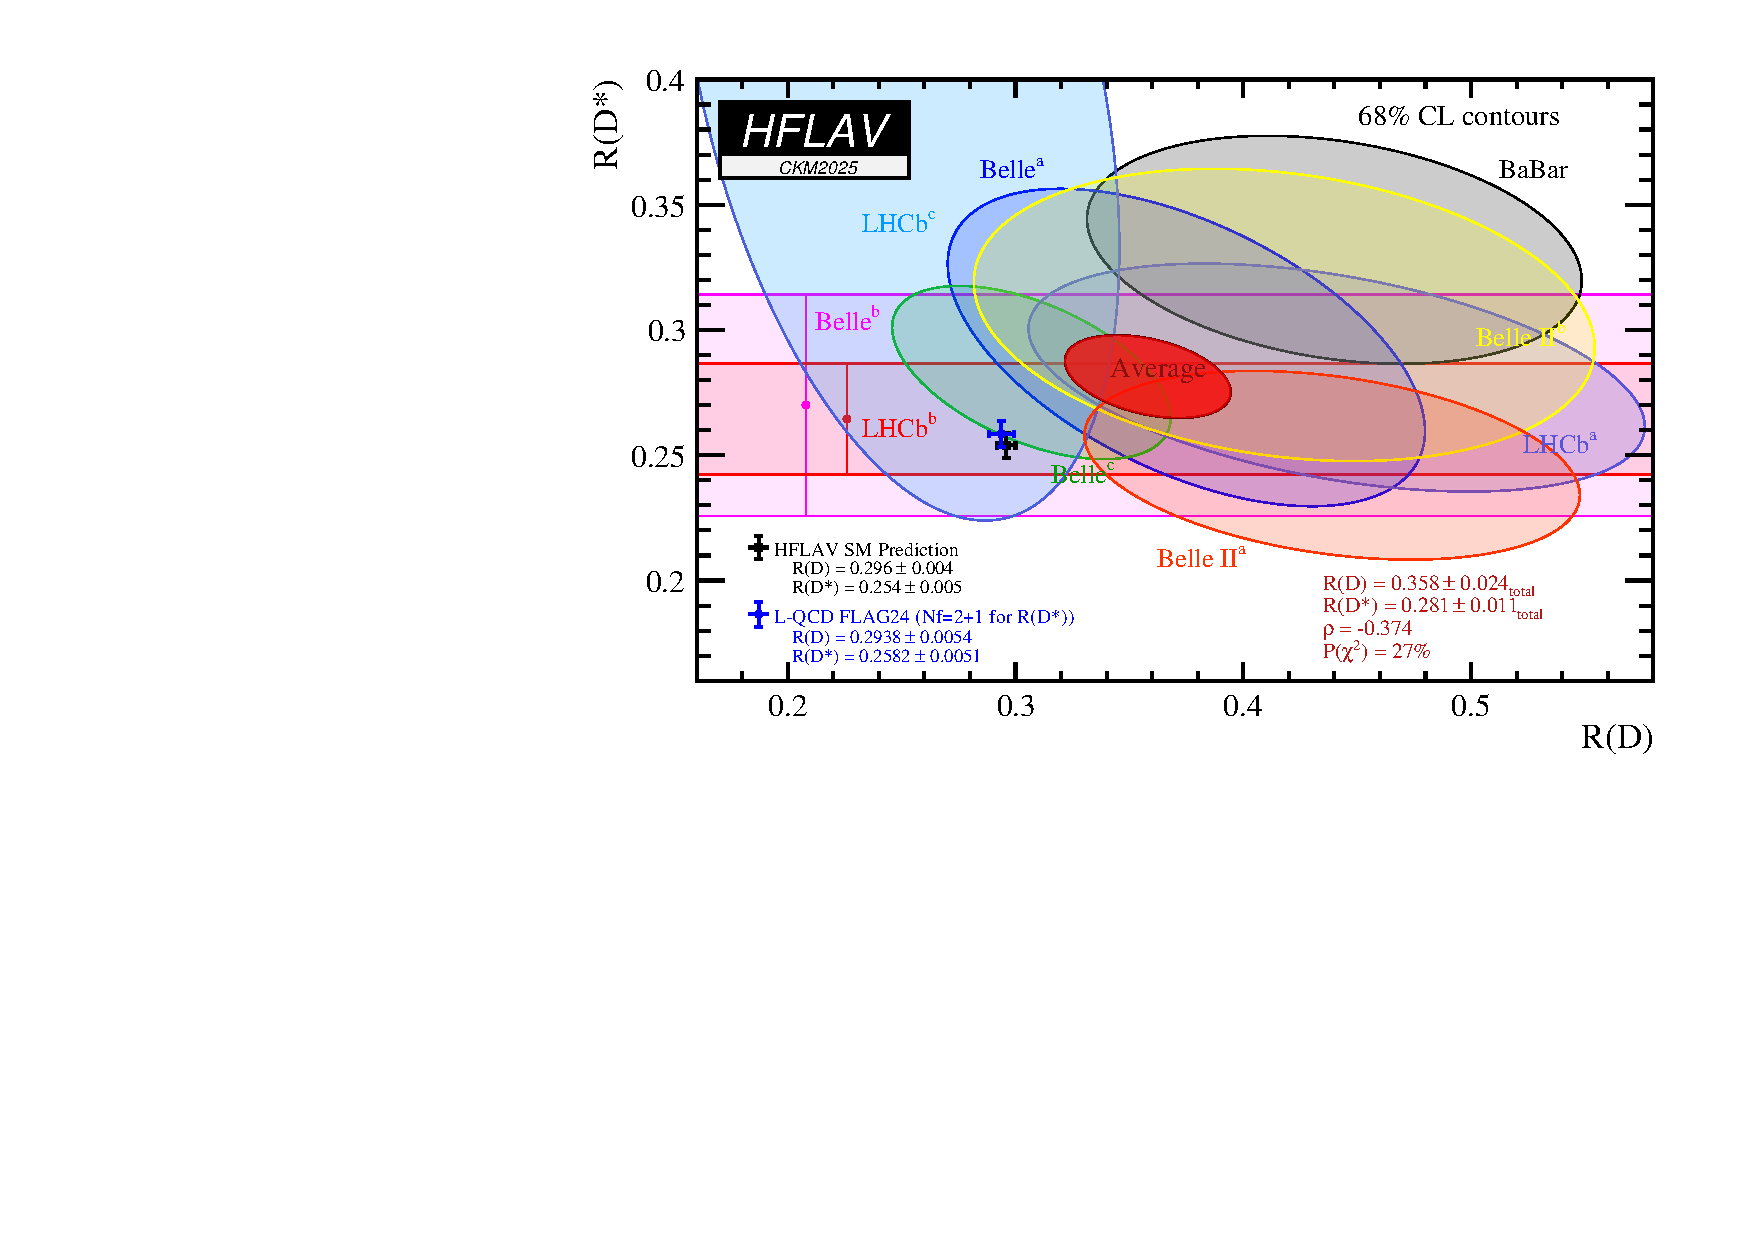
\includegraphics[width=0.75\linewidth]{Figs/CH2/rdrds_ckm2025_new.pdf}
    \caption[Average of $R(D^{*})$ and $R(D)$]{Average of $R(D^{*})$ and $R(D)$~\cite{HFLAV2025RDstar} measured by the BaBar~\cite{BaBar:2012obs, BaBar:2013mob}, Belle~\cite{Belle:2015qfa, Belle:2016dyj, Belle:2017ilt, Belle:2019rba}, Belle-II~\cite{Belle-II:2024ami, Belle-II:2025yjp}, and LHCb~\cite{LHCb:2023zxo, LHCb:2023uiv, LHCb:2024jll} experiments.}
    \label{fig:HFLAV2025}
\end{figure}


\section{Possible Solutions to the Remaining Problems of the Standard Model}
\label{sec:bsm_solutions}

Many extensions of the SM have been proposed to address one or more of the problems described above. 
This section briefly introduces several representative ideas: supersymmetry, axions, and leptoquarks. 
These models are not mutually exclusive, and in many cases they address different aspects of the SM's limitations.

\subsection{Supersymmetry}
\label{subsec:susy}

Supersymmetry~(SUSY) is a spacetime symmetry relating bosons and fermions~\cite{WessZumino1974,MartinSUSYPrimer}.
In supersymmetric theories, each SM particle is accompanied by a superpartner whose spin differs by one half unit.
The fermionic superpartners of bosons are conventionally named by adding the suffix `-ino', such as the gluino, wino, bino, and higgsino, while the bosonic superpartners of fermions are named by adding the prefix `s-', such as squarks and sleptons.
If supersymmetry were exact, particles and their superpartners would have equal masses.
Since no such superpartners have been observed, SUSY must be broken if it is realised in nature.

One of the main motivations for SUSY is the hierarchy problem.
Loop corrections to the Higgs mass from SM particles can be cancelled by corresponding contributions from their superpartners, reducing the sensitivity of the electroweak scale to very high energy scales~\cite{DimopoulosGeorgi1981,MartinSUSYPrimer}.
In models with conserved $R$-parity, supersymmetric particles are produced in pairs and the lightest supersymmetric particle~(LSP) is stable~\cite{FarrarFayet1978,MartinSUSYPrimer}.
If the LSP is electrically neutral and weakly interacting, such as a neutralino in many SUSY scenarios, it can provide a dark matter candidate~\cite{Goldberg1983,EllisOliveSantosoSpanos1984}.
SUSY can also improve the unification of gauge couplings at high energy, since the additional superpartners modify the renormalisation-group evolution of the gauge couplings~\cite{DimopoulosRabyWilczek1981,Amaldi1991}.
However, no direct evidence for supersymmetric particles has yet been observed, and the simplest low-scale SUSY scenarios are increasingly constrained by collider searches~\cite{ATLAS2024SUSYSummary}.

\subsection{Axions and the strong CP problem}
\label{subsec:axion}

The Peccei--Quinn mechanism provides a dynamical solution to the strong CP problem~\cite{PecceiQuinn1977PRL,PecceiQuinn1977PRD}. 
It introduces a new global chiral symmetry, usually denoted as the Peccei--Quinn symmetry $U(1)_{\mathrm{PQ}}$, which is spontaneously broken.
The associated pseudo-Nambu--Goldstone boson is the axion~\cite{Weinberg1978Axion,Wilczek1978Axion}. 
The axion field dynamically relaxes the effective value of $\bar{\theta}$ to zero, thereby explaining the absence of observable strong CP violation. 
In many models, axions or axion-like particles can also contribute to the dark matter density of the universe~\cite{KimCarosi2010}.

\subsection{Leptoquarks}
\label{subsec:leptoquarks_motivation}

Leptoquarks provide another well-motivated class of particles beyond the Standard Model. 
They are hypothetical bosons that couple directly to a quark and a lepton, thereby connecting the quark and lepton sectors. 
Such particles appear naturally in several extensions of the SM, including models based on quark--lepton unification, such as the Pati--Salam framework~\cite{PatiSalam1974}. 

Leptoquarks are particularly interesting because they can affect semileptonic processes. 
This makes them relevant to the flavour anomalies observed in several $B$-meson decay measurements, where the experimental results have shown tensions with the SM predictions in observables testing lepton-flavour universality. 

Among the possible leptoquark scenarios, the vector singlet leptoquark $U_{1}$ is especially well motivated for charged-current anomalies such as $b\rightarrow c\tau\nu$. 
This motivates collider searches for final states containing hadronically decaying $\tau$ leptons. 
The following chapter introduces the leptoquark models in more detail and the leptoquark searches at the LHC.
